%% This is an example first chapter.  You should put chapter/appendix that you
%% write into a separate file, and add a line \include{yourfilename} to
%% main.tex, where `yourfilename.tex' is the name of the chapter/appendix file.
%% You can process specific files by typing their names in at the 
%% \files=
%% prompt when you run the file main.tex through LaTeX.
\chapter{Soft Objects}
	
	\begin{center}
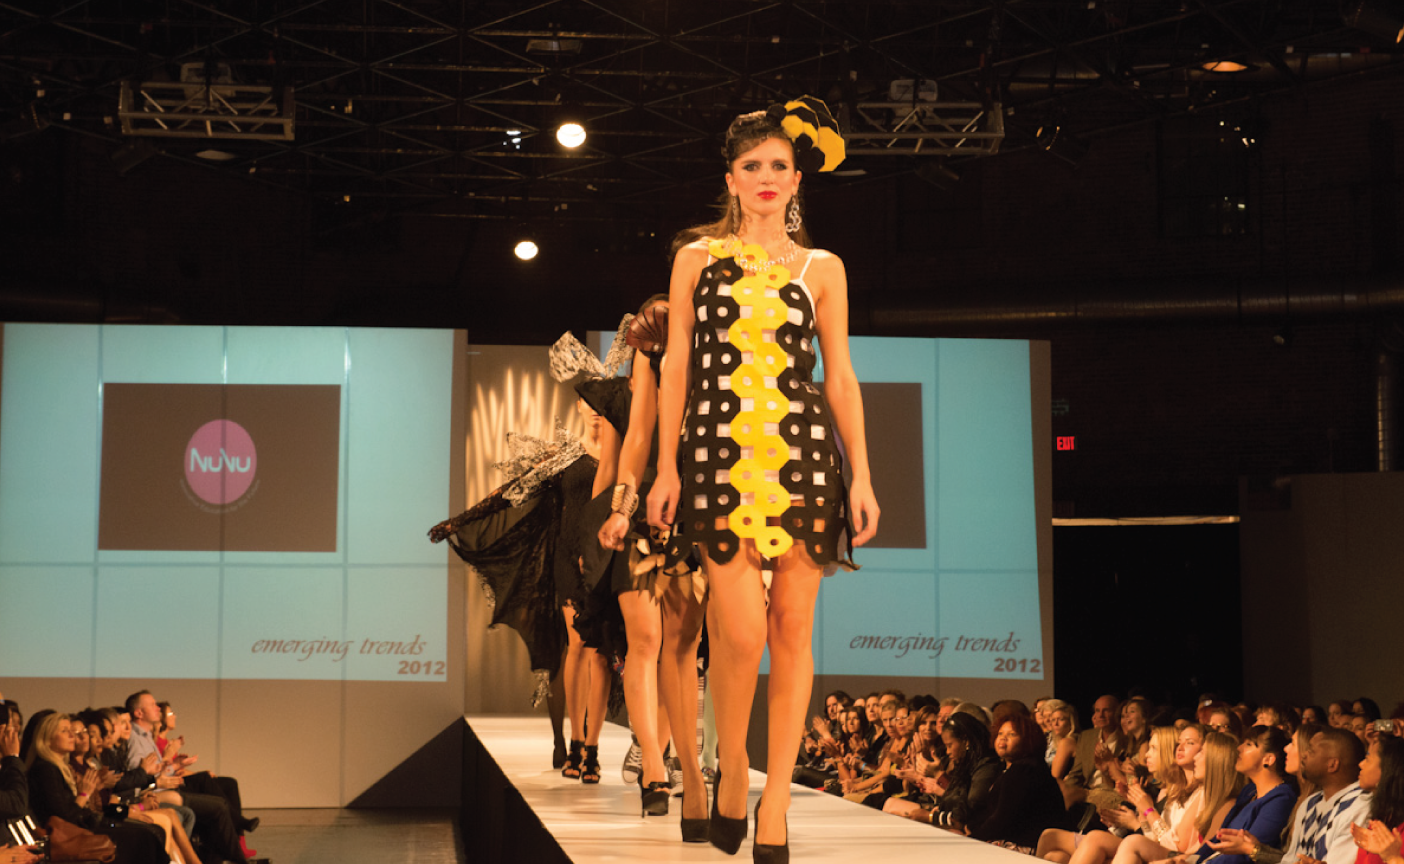
\includegraphics[width=6.5in]{images/fashion_show.png}
\end{center}
	
After an evaluation of the successes and limitations of the Codeable Objects library I made an effort to expand the library in a way that would allow for a broader range of computational design approaches and end products. In particular, I was interested in exploring the domain of algorithmically crafted garments and fashion accessories. To explore computational fashion design in the context of algorithm craft, I expanded the Codeable Objects tool into a more general programing library named SoftObjects and evaluated it over a 10 day workshop with young people.


\section{Motivation}
Fashion is an exiting domain to connect to computation, because it appeals to groups of people who are often under-represented in computer science, particularly women and girls. In addition, because garments and accessories are wearable, computational fashion design requires the programmer to consider questions of comfort, sizing and personal taste and and style; a set of concerns not often associated with most computer programs. With the growth public awareness of digital fabrication, there is particular enthusiasm for the wearable applications of emerging digital fabrication technology. Much of this excitement is directed towards 3D printed wearables and textiles. In July 2010, Iris Van Herpen released her Crystallization collection, which featured her first computationally designed, 3D printed piece, marking the first time a 3d printed garment had appeared on the runway \cite{herpen}. Herpen and many other fashion designers have continued using 3d printing as a medium for fashion since then. As a result, often in popular culture, computationally designed, digitally fabricated fashion is often synonymous with 3D printing. The 3D printed garments and accessories produced by professional designers like Van Herpen serve as wonderful inspiration for the future of digital fabrication, as they produce garments that would be impossible to fabricate through any other means. For the average individual however, computationally designed and digitally fabricated garments of this nature present significant limitations. Given current technology and material limitations, the majority of 3D printed garments are generally practical for every-day wear and require advanced fabrication techniques that are unavailable to the average designer. Garments like the N.12 bikini, designed by Continuum \cite{n12} are designed to be more practical, and available to consumers, however they still come at a steep price point (\$300 for the bikini top). Most importantly however, the construction of 3D printed garments of this nature, both in terms of materials and techniques, appear to have little in common with methods of traditional garment production, such as sewing, knitting and embroidery, and therefore offers few entry points to individuals with traditional skills to move into this space.

\begin{center}
\begin{figure}[h!]
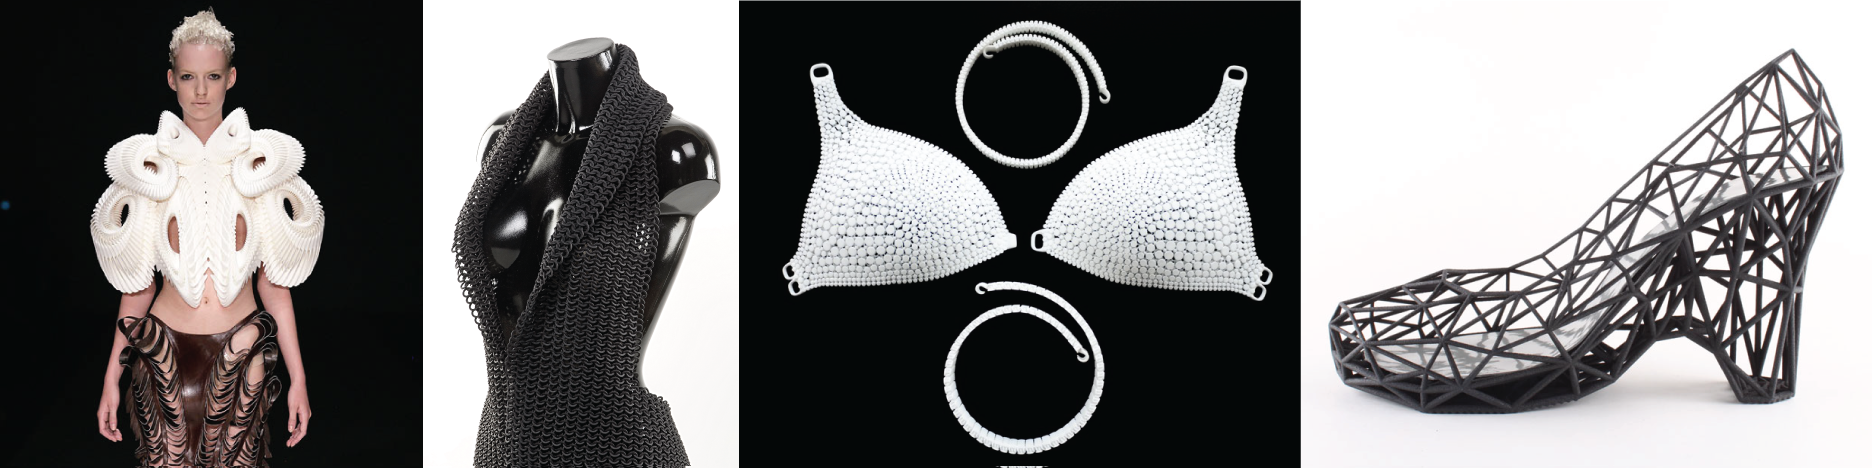
\includegraphics[width=6.5in]{images/3d_prinited_high_fashion.png}
\caption{ 3D printed fashion (from left to right: Crystallization 3d Top by Iris Van Herpen, Drape Dress by Janne Kyttanen, N12 Bikini by Continuum Fashion, Strvct shoe by Continuum Fashion}
\label{fig:high_fashion}
\end{figure}
\end{center}

Although perhaps less publicized than 3D printed fashion, other other designers are merging fashion with computation and digital fabrication in more accessible forms. Diana Eng's Laser Lace tee collection contains laser-cut machine-washable t-shirts with floral-inspired iconography, and her Fibonacci scarf is created through traditional knitting techniques, meshed with a Fibonacci knit pattern. Eunsuk Hur's modular fashion pieces are inspired by tessellations and fractal geometry, but apply these structures for a practical end as well. By creating garments through laser-cut interlocking pieces, Hur's aim was to produce items that were robust and durable, also gave the user the opportunity to use their inner creativity to come up with new and interesting items, by rearranging the individual components (figure:\ref{accessible_fashion}.)

Examples such as these demonstrate a space in computational fashion design that is open to a broader range of participation and compatible a larger set of interests, and skillsets. In general, less novel fabrication machines, like laser cutters and vinyl cutters are dominant in this type of work, because they afford a wider range of materials and can produce garments at a much lower cost than 3D printers. This range of materials also translates to a wider set of possibilities for aesthetics and styles than most forms of 3D printing. It should be noted that accessible forms of 3D printing can produce compelling wearable objects, however they are generally on the scale of jewelry and small accessories. As a whole, garments designed and produced in this fashion fit more so with the parameters algorithmic craft, than the 3D printed high-fashion examples provided in the preceding paragraph. With this distinction in mind, I developed the Soft Objects programming library, and designed and conducted a workshop to explore the creative potential of computation and digital fabrication in the context of accessible and immediate fashion design.

\begin{center}
\begin{figure}[h!]
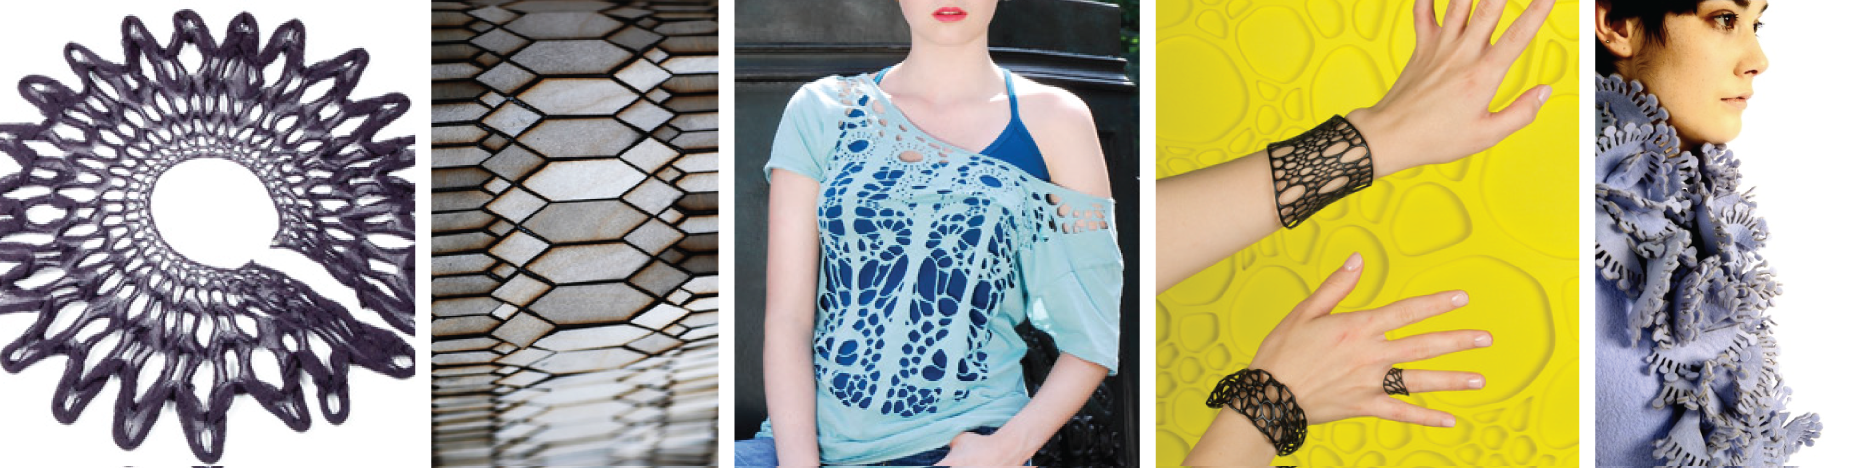
\includegraphics[width=6.5in]{images/accessible_fashion.png}
\caption{"Ready to wear" computational fashion (from left to right: Fibonacci Scarf by Diana Eng, Biomimicry laser-cut bracelet by Stefanie Nieuwenhuyse, Laser Lace All-Over Tee by Diana Eng,  Interstice bracelet by Nervous Systems, Modular Fashion by Eunsuk Hur}
\label{fig:accessible_fashion}
\end{figure}
\end{center}
		

\section{Tool description}
The Soft Objects library contains a set of methods that allows users to draw shapes and patterns and then export those shapes and patterns in a vector-file format that is compatible with x-y axis digital-fabrication machines. Similar to CodeableObjects, to use the library, a user imports it into the Processing environment and then writes and compiles code using the Processing editor. Soft Objects allows users to define and manipulate basic geometric primitives such as Points, Lines, Curves and Polygons. These primitives can then be collected within Pattern and Shape objects�structures designed to capture surface decoration and 2D structure, respectively�to form increasingly complex designs. 

Soft Objects is formulated on an Object Oriented Programming (OOP) paradigm, which lets users create and manipulate collections of geometric primitives�Patterns and Shapes. This structure differs from Processing�s drawing API, which uses a functional programing approach. The structure of Soft Objects enables users to simultaneously apply transformations to all of the elements in a collection that make up a complex pattern or shape. It is also possible to import scalar vector graphics files (SVGs) to incorporate pre-drawn designs as elements within a pattern or as a container for existing patterns.

\begin{center}
\begin{figure}[h!]
\fbox{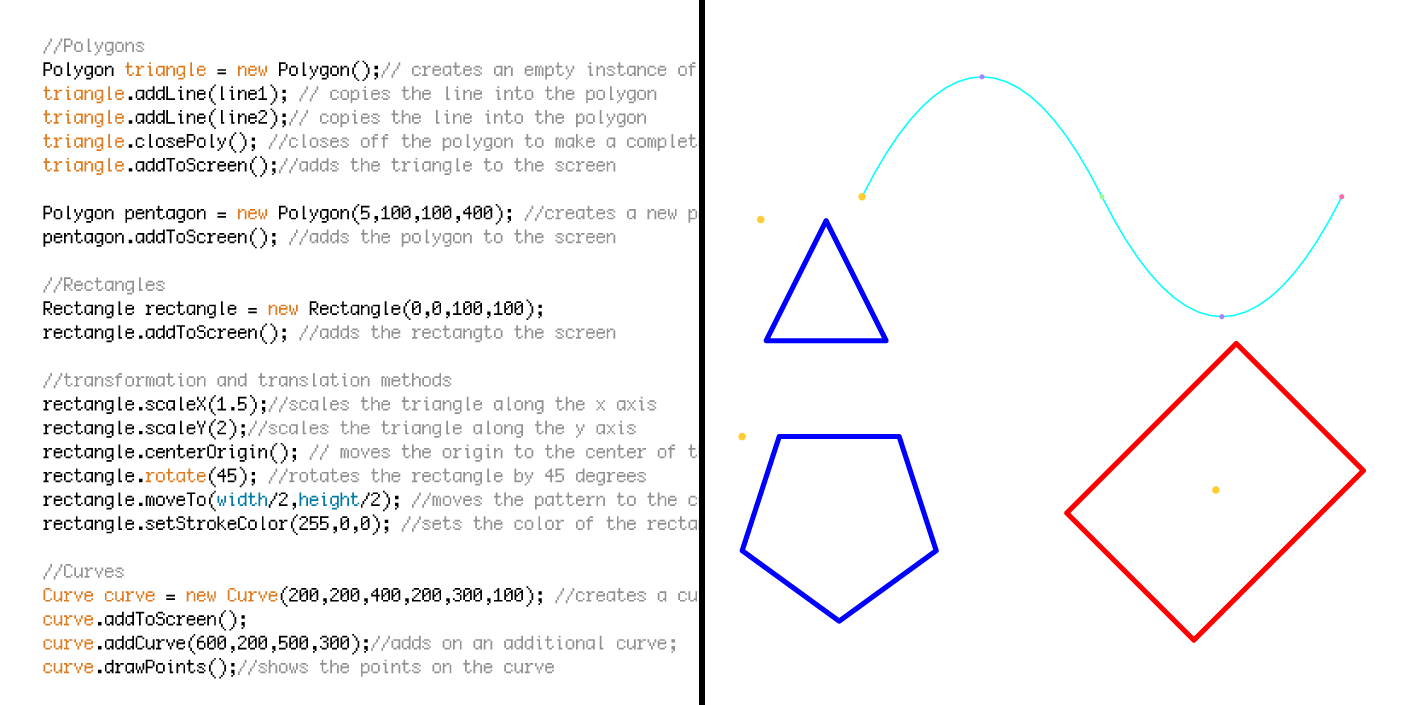
\includegraphics[width=6.5in]{images/primitive_syntax.png}}
\caption{Soft Objects primitives}
\label{fig:softobjects_primitives}
\end{figure}
\end{center}
		

Users are presented with a 2D preview of their designs when they compile their code. Soft Objects supports a variety of digital-fabrication machines by allowing users to save designs to vector portable document format (PDF) files. PDFs can be used by different production tools, including ink-jet printers, vinyl cutters, laser cutters, and computationally controlled embroidery machines. Output from Soft Objects can be fabricated on essentially any x-y axis tool. 3D structures can be created by assembling fabricated pieces. Figure \ref{fig:softobjects_workflow} demonstrates the workflow from code to a finished object. 
The Soft Objects library also contains a collection of pre-defined algorithmic patterns that can be initialized, including Voronoi diagrams, Koch curves, and L-Systems, and an extensive set of example programs that users can modify and combine to produce individual results.		

\begin{center}
\begin{figure}[h!]
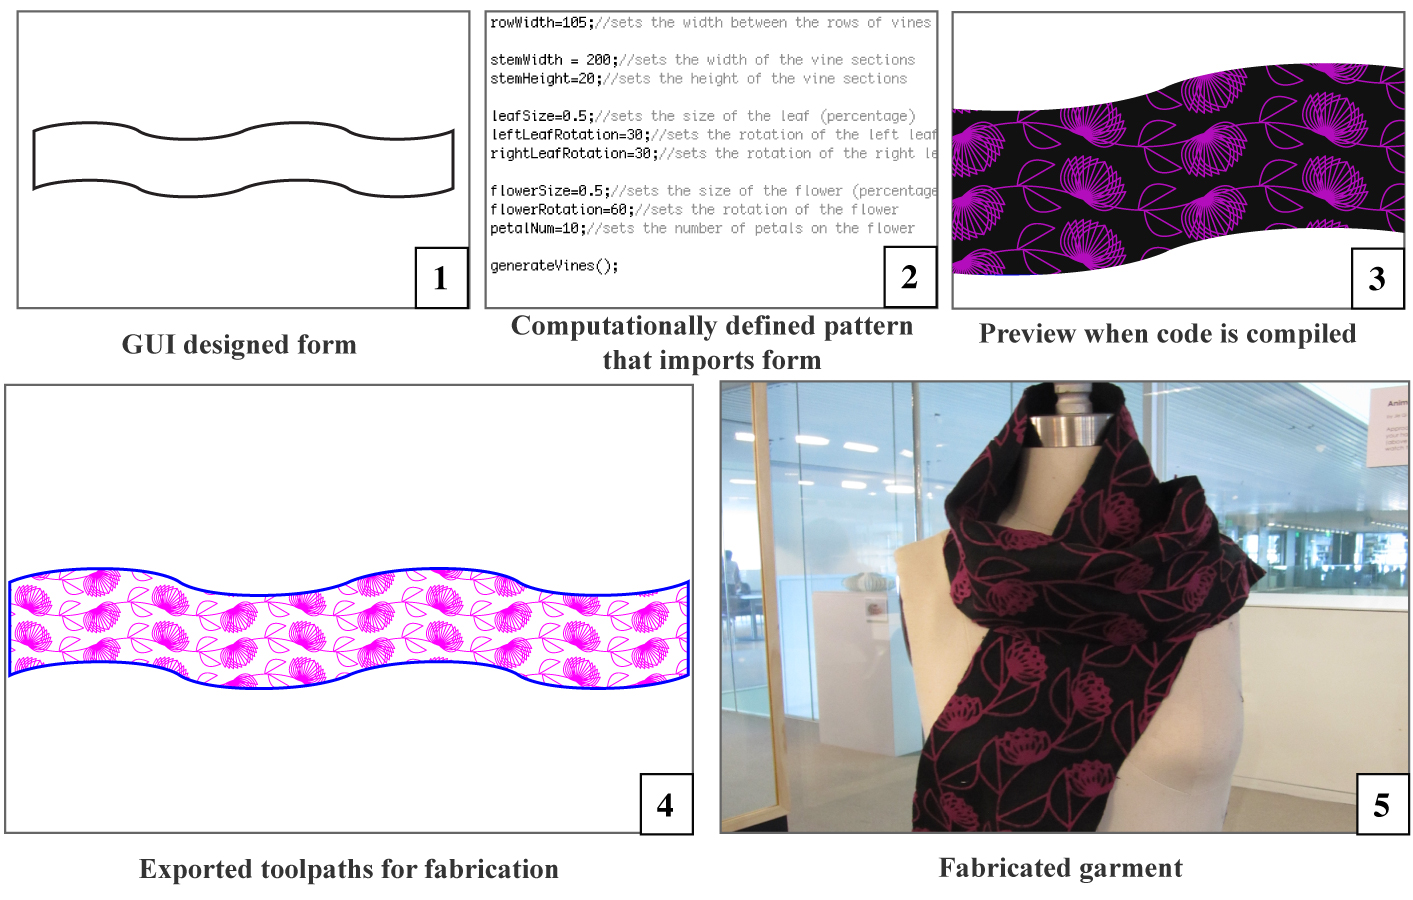
\includegraphics[width=6.5in]{images/softobjects_workflow.jpg}
\caption{Soft Objects workflow}
\label{fig:softobjects_workflow}
\end{figure}
\end{center}
		
\section{Workshop}
The evaluation of Soft Objects was conducted during a 10-day workshop with a representative group of participants�eight young adults, aged 11-17, 75\% male and 25\% female. A significant majority (88\%) stated in pre-surveys that they had little or no prior experience in programming, and only one participant had prior experience in Processing. All of the participants indicated some level of prior experience in art, design, or craft. Most attributed their design or craft experience to art or drawing classes.

The workshop was conducted at the Nuvu Magnet Innovation Center for Young Minds. Participants were given 10 days to conceptualize and construct a garment using a combination of computational design, digital fabrication, and traditional sewing and crafting. The second study was more open than the first; participants could produce any type of garment they wished as long as components of it were computationally designed and digitally fabricated. During the workshop, participants were introduced to Soft Objects and the concept of computational fashion through a multi-step process that engaged participants in different levels of programming through the construction of different garments and accessories. First, participants were provided with a small set of example programs similar to the lamp workshop. This step allowed them to manipulate a core set of parameters to generate the pattern and form of a scarf, which they then cut on the laser cutter (figure: \ref{fig:scarves_bracelets}.) 

\begin{center}
\begin{figure}[h!]
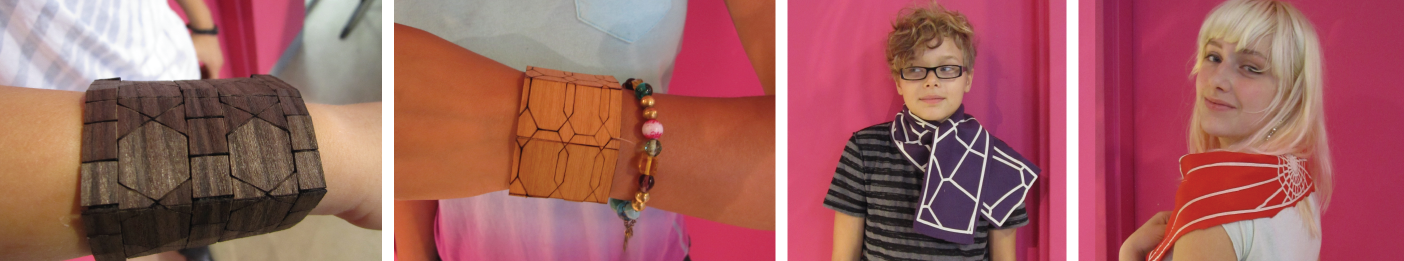
\includegraphics[width=6.5in]{images/scarves_bracelets.png}
\caption{Completed garments (from left to right: octagon dress, flag pants, samurai dress, viral sweatshirt)}
\label{fig:scarves_bracelets}
\end{figure}
\end{center}


Second, participants were instructed in a number of primary programing concepts, including iteration, function definition, and the use of variables and primitive data-types. During this instruction, participants were guided through the process of independently using Soft Objects and generating their own programs from scratch. They used these programs to create a design for a wooden bracelet (Fig. 3), which was then laser cut and assembled. After these two initiation activities, these participants were asked to conceive their own garments and provided with the resources to design, prototype, and craft finished garments.


\section{Results}
Participants in the fashion workshop were successful in using programing and digital fabrication to design and produce finished garments. During the initiation activities, participants independently wrote and compiled programs of their own and produced physical products based on the design generated from that program. Furthermore, with assistance from the instructors, the participants were able to apply more sophisticated programing methods to produce a diverse set of final products (Fig 4). One pair of students developed an �armor dress� by writing a program that geometrically described a single �scale� shape, imported a dress pattern from Illustrator and filled it with rows of scales that corresponded with the dimensions of the dress. Another pair created a geometrically inspired dress with a patterning of different-sized octagons and squares that were laser cut from starched fabric. Another student created American-flag-inspired pants using a program that generated random orderings of red and blue stripes on a white background. One group that was less interested in the process of sewing clothing created a program that generated a recursive virus-like pattern and then screen-printed the pattern on pre-made sweatshirts and t-shirts. 

\begin{center}
\begin{figure}[h!]
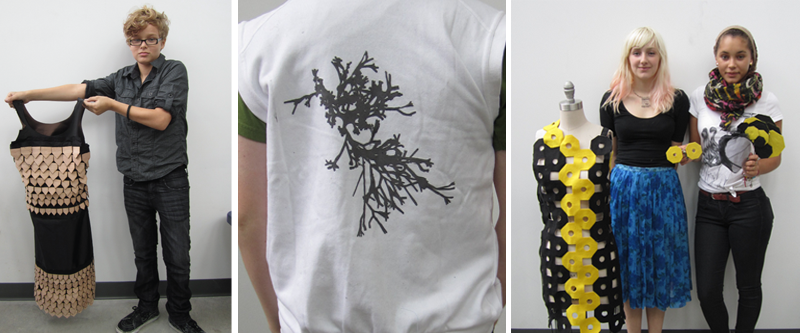
\includegraphics[width=6.5in]{images/fashion_results.png}
\caption{Bracelets and scarves from preliminary activities}
\label{fig:fashion_results}
\end{figure}
\end{center}


On the post survey, when asked if they �were able to complete a finished project to their satisfaction,� 100\% of the fashion participants responded yes. The resultant garments were attractive and functional, indicated by the fact that participants from the fashion workshop kept and wore their creations. Direct comparison of the pre-and post-workshop surveys also demonstrated that on average, participants in the fashion workshop indicated their interest in crafting increased after the workshop, as did their enjoyment of the design process. Eighty-eight percent of the participants in the fashion workshop indicated that they felt more comfortable programing after the workshop than before.

\section{Discussion}
The Fashion workshop occurred over a longer time period than the Lamp workshop, and explored a wider range of crafting and computational techniques. As a result, I had an opportunity to spend greater amounts of time observing and talking with the  participants. leading to a more comprehensive perspective on the benefits and challenges in conducting algorithmic craft  workshops. In addition, because the participants were nascent programers, their experiences better reflect those of the target demographic of this research. Through this workshop we confirmed that algorithmic craft activities can actively support the expression of personal identity in a positive setting. It can also foster feelings of confidence in programming and support aesthetic and technological literacy. The workshop also promoted a deep understanding of computation as evidenced by critiques of the participants as well as demonstrating the importance of physical prototypes in the design process. Finally, the workshop promoted a sustained engagement in programing. The evidence of these outcomes is discussed in greater detail below

 
\subsection{Identification as a programmer}
Similar to the participants in the Lamp workshop, the Fashion participants began with vague ideas about the applications of computation. When asked in the pre-workshop surveys how they thought programing, art and craft could be combined, participants responded in writing in the following ways:

\textit{"To be honest, I am not sure too sure how it would all be combined because I don't know much about programming."} [Fashion Participant Y]

\textit{"With programing, we can make programs do things for us. "}[Fashion Participant J]

In addition, the participants had almost no prior knowledge of computational design. Those participants who had some form of prior programing experience associated it largely with interactivity and actuation:

\textit{"I would love to combine things like T-shirts and speakers or other different types of technologies. "}
[Fashion Participant J]

Following the completion of their final projects, participants were much more descriptive about the applications of programing:

\textit{"I think [programing and fashion] are really interesting but I never thought they could ever be together in one concept, and it�s awesome that I know that now- that you can design aesthetically pleasing things from coding."}
[Fashion participant K]

\textit{"I�ve never thought of programing as physical, I thought it was only in computers. But then when we made the scarves and stuff, I thought that was really fun."}
[Fashion participant M]

In addition, they expressed a growing confidence in their ability as programmers. During the interviews, several separately stated that that while they did not feel completely comfortable programing independently, the experience made programming feel significantly more accessible:

\textit{"For someone who never had any programing explained to them before, when you look at [computational drawing examples] it feels really inaccessible, but now that I�ve been taught a little bit of [programing], I can kind of crack at the walls a little bit and understand how it works, and that makes it more accessible to me."}
[Fashion participant S]

\textit{"Even though now I�m not really a Processing expert now, I�ve just experienced it and it�s not as scary to me, like the idea of coding, you just kind of have to learn some stuff and practice it more, but I think I definitely understand the concept of it. [Fashion participant K]"}

Finally, the programmers in the fashion workshop expressed feelings of pride and a sense of accomplishment in their new-found programing skills:

\textit{''I�m actually kind of proud. I know what�s going on. It feels different�I just thought [programming] was just about these huge programs that you have to piece together, and that you have to be really, really smart to do it, but I can do it."} [Fashion participant P]

\textit{"I think it was really cool that we used [programing] for fashion, cause I think a lot of people might think people who do fashion aren�t really smart or something, and then they think that people who design code are like brilliant coders and can do really awesome stuff with it."}
[Fashion participant K]

 The confidence, sense of belonging, and personal agency demonstrated in these comments stand in contrast to popular views of programming as specialized and inaccessible. These sentiments were also present in later workshops I conducted with other nascent programmers (discussed in the section \ref{sec:DressCode}), indicating that introducing programing in the context of algorithmic crafting not only has the potential to change people�s understanding of the relevance and applications of programing, but also promote a personal awareness of technological literacy and competence. 
 
\subsection{Application of computational affordances}
Aside from a general understanding of the potential applications of programing, participants were successfully able to leverage the advantages of computational design in their final projects. For example, the octagon dress used parametric design principles as the participants were able to change the size and orientation of the octagons in the dress by modifying several parameters at the start of their program to affect the entire pattern, rather than rotating and adjusting each shape independently. The samurai dress took advantage of the computational properties of precision and automation. With help from an instructor, the creators programmatically generated an individual vector file for each row of scales of the dress, expediting the production process (figure:\ref{fig:samurai_dress_progression}.)The samurai dress is particularly interesting because it shows a remarkably successful transition from the design expressed in original concept art by the participant, and the resultant garment. In later workshops it was often difficult to reconcile the sketched concepts with the qualities of computational design. Lastly, the viral shirt, demonstrated an application of generativity. The aesthetic of the viral pattern was produced through the use of a weighted random-number generator to determine the number and length of the branches in each recursion of the pattern. Although the implementation of the weighted number generator was facilitated through the help of the instructor, the participants came up with the idea of using it on their own.
\begin{center}
\begin{figure}[h!]
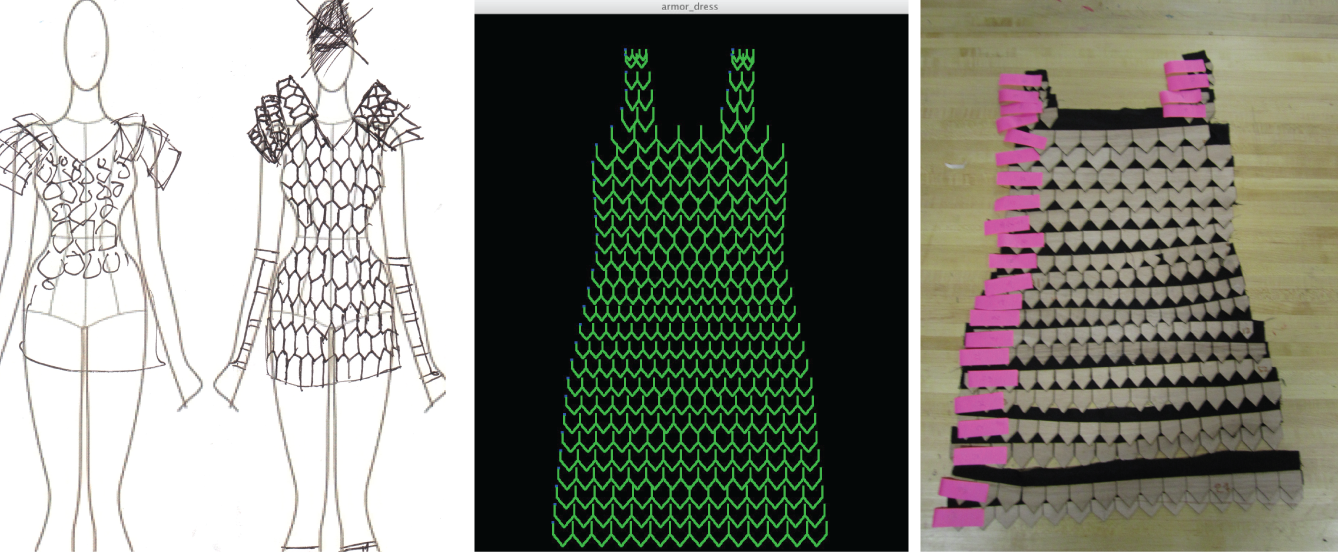
\includegraphics[width=6.5in]{images/samurai_dress_progression.png}
\caption{Progression of samurai dress (from left to right: concept sketch, computationally generated pattern,laser-cut components of final garment)}
\label{fig:samurai_dress_progression}
\end{figure}
\end{center}

Aside from conceiving of and applying computational-design approaches, participants demonstrated an understanding of the rationale behind the methods they were using. One of the participants in the armor dress project compared the process of programing the design of the dress to that of manually drawing it: 

\textit{''With drawing you can achieve everything programing can, but I would prefer to program it. [Programing] can be pretty convenient�the computer is helping me. Like if you want to make pizza, the computer is like a pre-made crust."}[Fashion participant E]

Participants also demonstrated an understanding of specific programing functionality. One participant described the point at which she understood the application 
of parameterization:

\textit{''One moment that stuck out was when you helped me make a code with original geometry that could be changed so that when you changed one thing it changed everything and that was cool because I felt like I actually made something that could be changed and then applied."}
[Fashion participant K]

The ability to understand and describe how computational support one's creative objectives is essential in motivating an individual to spend time learning and implementing these methods. Once the aesthetic possibilities of the recursive viral pattern were apparent to the designers, they became engaged in better understanding the underlying algorithm, so that they could produce a pattern to their exact specifications. Conversely the participants were far less engaged during several of the introductory lessons when we introduced several elementary computational principles, such as defining data types, where it was unclear what the immediate design application was. Algorithmic craft presents the opportunity for participants to tackle complex computational problems with sophisticated approaches, however the problems themselves must be clearly grounded within the design objectives of the individual. One of the challenges in engaging new programmers in Algorithmic craft therefore, is in selecting programing approaches that allow for compelling aesthetic and design possibilities, but are also approachable for first-time coders. 

\subsection{Aesthetics and Identity Expressed through Code}
The fashion workshop provided the opportunity for participants to use computational aesthetics as a way to express their visual identity. Fashion can serve as a means of self-expression and for conveying one�s identity. Discussions of fashion conducted with the participants of the second workshop indicated that participants were aware of the connection between fashion and identity and were eager for opportunities to create clothes that expressed their style. As a result, the majority of the garments created in the workshop contained an expression of the �fashion sense� of the participants who created them. For example, the participant who created the flag pants was very explicit that the pants have some form of an American flag motif, but not resemble the traditional, and as he put it �tacky� flag pants that he commonly saw. He wanted his flag pants to be as he put it �something that he would actually want to wear.� His programing choices were made in direct consideration of his desire to create a pair of pants that he felt were �fashionable.� 

When asked about the experience of making and designing his pants he said:

\textit{''[The workshop] definitely changed my impression of making clothes, I thought it was pretty quick to make clothes, but it actually takes a long time, and it�s also really fun. I love the fabric I made."} [Fashion participant M]

His enthusiasm also was evident in the fact that after the pants were complete, he tried them on and wore them for the remainder of the workshop. This level of enthusiasm was common among participants; they all proudly modeled their creations, and many of them wore them home. This behavior suggests a relationship between the decisions made in a programing context, and the participant�s desires to express their visual identity. The participants were selective in the code they wrote to design their garments because they intended to wear the garments, and as a result, be represented by them. This powerful affective relationship between computation, design and self-expression provides a natural way to engage people in programing and design by supporting their personal interests. 

\subsection{Physical and Digital connections}

One of the challenges of Algorithmic Craft, alluded to in the Codeable Objects discussion, is that the practitioner must work between digital designs with physical materials and processes.  Physical prototypes often serve as a key point of transition between these spaces. In the fashion workshop, prototyping played an important role, and demonstrated how computational tools can support and sometimes hinder the prototyping process. The focus on fashion made it possible to supply the participants with large amounts of inexpensive test fabric. The laser cutter could cut fabric much more quickly than thick materials, which allowed participants to produce numerous prototypes of their projects before creating a final piece. Most groups produced two or three prototypes, with one participant creating six iterations of a single jacket. This rapid production process formed a direct connection between discoveries made in the physical prototyping space and decisions in the programing realm. 
In the case of the octagon dress, (figure:\ref{fig:fashion_results}), the participants first cut test rows of octagons to determine the appropriate scale, then adjusted their design by modifying their program. When they had cut out a second more complete version of the dress, they rotated one of the shoulder straps on the physical prototype and formed an idea for a one-sided shoulder strap. They implemented this design change in the digital version of the dress by making additional changes to the size and rotation of the shapes defined in the code. When asked about this process in the interview one of the participants said:

\textit{''I think it was really fun that we got to do a prototype first because then if you don�t like it, you don�t feel a lot of pressure because you can make it again really fast, and there�s no stress because if it doesn�t turn out well, then it�s not your final project.} [Fashion Participant K]

The combination of programming, rapid fabrication, and physical construction allowed for a design approach that transitioned from programing to fabrication to programming adjustments based on the fabricated elements, and then back to fabrication. This iterative approach resulted in a closely linked cycle of physical and digital engagement. 

Despite these positive results, many participants struggled with prototyping. These struggles were  evident in practical aspects, such as participants not saving their programs and digital design files  to come back to later(despite repeated reminders from the instructors to do so). Participants also frequently spent too much time on assembling their early prototypes and were frustrated when they realized they would have to make design changes and repeat some of the manual labor. Although we took pains in the workshop to introduce participants to the concept of prototyping, these instructions were not always absorbed. This may present an opportunity for future algorithmic crafting tools to contain specific features to encourage and support the physical prototyping process. One possibility that is often proposed in the HCI community is to include simulation tools that preview the constraints and behaviors of physical materials. The value of working with physical prototypes should also be supported however, by features that allow the designer to scale their files and fabricate first in miniature, and software that allows easy access and management of multiple versions of a design throughout the design process.

 \subsection{Enthusiasm in crafting and coding}
One of the most encouraging aspects of following the fashion workshop, was the participant's enthusiasm and desire to continue making. Participants talked extensively about what they would like to make in future with programming, consisting citing that they would like to continue making clothing, or other personal functional items like furniture and �things they could use around the house.� The experience of both sets of workshop participants also demonstrated the ability of these techniques to produce objects that were designed to complement personal items and living spaces. When asked what she would like to make if she continued to program, one participant responded: 

\textit{''Things like we�re making now, things that you would want to keep or use, things that look nice as opposed to like computer games, or �input-output� devices. I think those are fun, but it�s not as cool as things that you can hold in your hand. I actually hung up the scarf I made in my room, and now I can be like �I made this on Processing� and people will be like what? It�s cool! "}[Fashion participant K]

This enthusiasm, combined with the high potential for individual expression and sense of accomplishment encouraged us to continue exploring fashion and garment production as topic space for algorithmic craft. While the fashion workshop highlighted many positives in this sense, we also encountered several areas for improvement. 

\section{Limitations}
The most evident barriers in the Fashion workshop involved the syntactic challenges of programming. Many participants expressed a frustration with the syntax in both surveys and in-person interviews. Although the workshop participants were able to generate their own programs, they required more assistance from an instructor to write some of the commands. In addition, a feeling of needing to memorize programming syntax frequently translated to a sense of frustration. One participant stated in an interview:

\textit{''I couldn�t memorize things, so it also was frustrating for me to always have to get you to help me write the code."} [Fashion participant K]

Many people requested some form of written "cheat sheet" that listed the key methods and how to use them. They also pointed out that you often had to write a lot of code (such as import commands and setup and draw functions), even for simple tasks. Writing code for the first time is always challenging, however, the high levels of frustration registered by the participants often focused on aspects of programming that seemed extraneous to design. Because we wrote Soft Objects as a Processing library, it required that the syntax correspond to Java, which is a difficult language for beginners. Because Java is a general application language, it has many syntactic requirements that are unnecessary for computational design applications. Based on this difficulty I concluded that future algorithmic crafting tools should explore domain-specific languages that directly applied to design and fabrication, and were better suited for first time programmers. 
 
Along with difficulties with the programing syntax, participants struggled with some of the post-processing techniques. In order to be suitable for digital fabrication, many of the participant's computationally generated designs required some processing in Adobe illustrator. Usually this required using illustrator's shape boolean functionality to merge shapes or expand outlines so that the vector paths would correspond to the desired cut pattern on the laser cutter (figure:\ref{fig:illustrator_example}.) Although the methods to perform these operations were simple, they needed to be repeated every time the design was modified programatically. This was not only inefficient, but sometimes prevented people from determining if their designs were feasible for fabrication when they were in the programing environment. This difficulty encouraged me to focus on ways of removing the need for illustrator from the process altogether so that all design modifications could be initialized and updated programatically.
\begin{center}
\begin{figure}[h!]

\includegraphics[width=6.5in]{images/illustrator_example.png}
\caption{Illustrator shape booleans - the laser cutter would cut along the blue line (from left to right: vector path, expanded vector path, group of individual vector polygons, merged group of vector polygons)}
\label{fig:illustrator_example}
\end{figure}
\end{center}
Finally, as in the Lamp workshop, participants were frustrated by the delay between adjusting their code and seeing the results. Although, not an absolute solution to the challenges in learning programing syntax, a programing environment with more immediate feedback could assist with the issue of syntactic challenges by providing novice users with improved ways to visualize the effect their syntactic changes have on their design. The implementation of background compiling, the process by which code is automatically compiled and executed as changes are made, has been applied successfully in several tools for novice programmers, including Scratch and Alice, and more recently with Khan Academy \cite{khan}. Our reliance on the Processing for Soft Objects made the incorporation of real-time compilation infeasible, however it quickly became a goal for future tools.


\todo{\subsection{Critiques of computational design}}
